\documentclass{article}
\usepackage[utf8]{inputenc}
\usepackage[a4paper, portrait, margin=1in, top=10mm]{geometry}
\usepackage{amsmath}
\usepackage{esvect}                                 %vectors
%\usepackage{siunitx}
\usepackage{tabularx,ragged2e,booktabs,caption}     %table
\usepackage{graphicx}                               %figures
\usepackage{tabu}                                   %matrix based table
%\usepackage{multirow}                               %multiple rows with different #of columns
%\usepackage{breqn}                                 %to break equations to multi-line
\usepackage{float}                                  %figure [H]
\usepackage{url}                                    %url's
%\usepackage{color}
%\usepackage{mathrsfs}


\begin{document}

\title{Project Proposal -  Simple Diode Model}
\author{Sonya Stuhec - Leonard 100963181}
\maketitle

\begin{figure}[H]
\centering
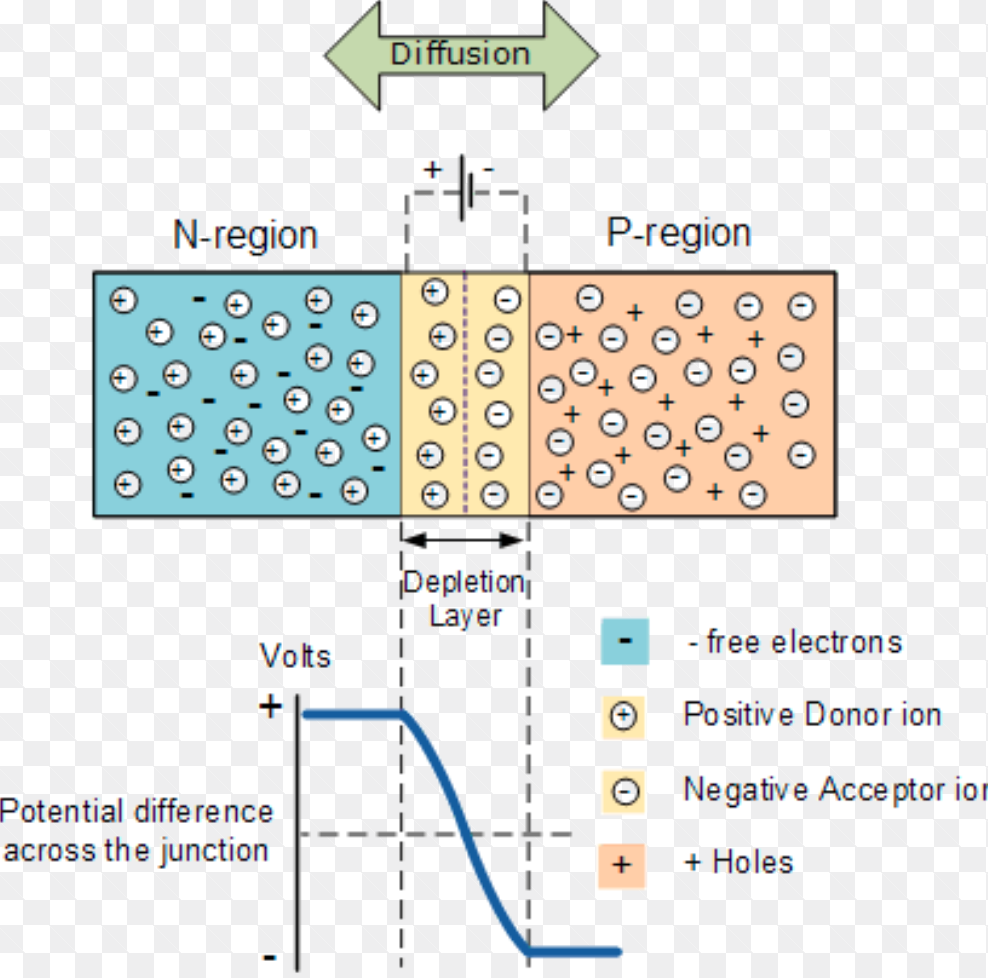
\includegraphics[scale=0.4]{DiodeModle}
\caption{Simple  diode modle depicting the idea for the project \cite{pic}}
\label{fig:pic}
\end{figure}

\section{The Model}
\begin{enumerate}
\item MC random initialization of electrons in the substrates
\item FD to move initialized electrons into equilibrium positions
\item Probability of leaving the depletion region and for entering based on state of electrons (when at equilibrium has minimal probability, perhaps simulate as zero)
\item Effect of applying an electric field in forward and reversed bias. Using FD to reach new equilibrium or steady state
\item Effect of applying an AC signal to the diode
\item MC generation of electrons with excess thermal energy, allowing them to penetrate the depletion region 
\end{enumerate}

\section{Deliverables}
\begin{enumerate}
\item Plot of electron trajectories
\item Force on each electron
\item Drift current calculation
\item Plot of electric field
\item Plot of temperature
\item Electron density map
\item Observe effects of changing threshold voltage
\item Plot electron velocity vs voltage (to see the effect of AC voltage)
\end{enumerate}

\begin{thebibliography}{9}
%\bibitem{hyper}Hyper Physics, \emph{Magnetic Interactions and the Lande' g-Factor}, [Accessed: January 8, 2017] WWW Document, (\url{http://hyperphysics.phy-astr.gsu.edu/hbase/quantum/Lande.html}).
\bibitem{pic} EduMission, "Physics Form 5: Chapter 4 - P-N Junction of Semiconductor" [Accessed: February 6, 2018] WWW Document,  (\url{http://cikguwong.blogspot.ca/2013/07/physics-form-5-chapter-4-p-n-junction.html})
\end{thebibliography}

\end{document}